\documentclass[../main]{subfiles}

\begin{document}

\chapter{A debugger for Scratch}\label{ch:blink}

%\dictum[B. Kernighan and P.\,J. Plauger \\ \textit{The Elements of Programming Style}]{
%    Everyone knows that debugging is twice as hard as writing a program in the first place. So if you're as
%    clever as you can be when you write it, how will you ever debug it?
%}

The process of teaching young students to code is often slowed down by the delay in providing feedback on each student's code.
Especially in larger classrooms, teachers often lack the time to give individual feedback to each student.
That is why it is important to equip students with tools that can provide immediate feedback and thus enhance their independent learning skills.
This chapter presents Blink, a debugging tool specifically designed for Scratch, the most commonly taught programming language for young students.
Blink comes with basic debugging features such as `step' and `pause', allowing precise monitoring of the execution of Scratch programs.
It also provides users with more advanced debugging options, such as back-in-time debugging and programmable pause.
A group of students attending an extracurricular coding class have been testing the usefulness of Blink.
Feedback from these young users indicates that Blink helps them pinpoint programming errors more accurately, and they have expressed an overall positive view of the tool.

\section{Motivation and significance}\label{sec:blink-motivation}

As society becomes increasingly digital, the demand for computer science education is also growing.
Current projections suggest that up to \qty{90}{\percent} of the workforce will need some level of digital skills to fulfil their professional responsibilities~\autocite{bejakovicImportanceDigitalLiteracy2020}.
A notable trend in European computer science education is the increasing integration of coding in the curriculum of both primary and secondary schools~\autocite{balanskatComputingOurFuture2015}.
Countries such as Estonia, France, Spain, Slovakia, and the United Kingdom are leading the way in this integration.

With the increasing emphasis on computer science education, the need for effective tools to facilitate coding education has also grown.
The Lifelong Kindergarten group at MIT has played a crucial role in this area by developing Scratch~\autocite{resnickScratchProgrammingAll2009}, an introduction of which is given in \cref{ch:scratch-the-programming-environment}.
Many computer science curricula have adopted Scratch to teach students the basics of computer science, as it is a useful tool for teaching computational thinking concepts~\autocite{zhangSystematicReviewLearning2019}.

As students navigate the programming landscape, they will inevitably encounter bugs that cause unexpected behaviour during code execution~\autocite{zellerWhyProgramsFail2009}, and Scratch is no exception.
The difficulty in detecting the root cause of a failure is that when a bug is activated, the system will arrive in an erroneous state but might still behave as expected.
It is only later when this erroneous state is propagated throughout the system that the system will reach a state that is observably wrong, leading to a failure~\autocite{ammannIntroductionSoftwareTesting2016}.
Additionally, Scratch uses a ``failsoft'' mode: errors are often swallowed, and execution continues without notifying the user~\autocite{hromkovicProblemDebuggingCurrent2021}.
Starting from the failure and working backwards to find the bug can be a daunting task, especially in larger or more complex programs.

In a classroom setting, the onus often falls on the teacher to guide students in identifying these bugs.
However, the inherent flexibility of programming -- where different code can produce the same result -- makes this a labour-intensive task for teachers~\autocite{kimDebuggingBlockbasedProgramming2018}.
A tool that makes it easier for students to identify errors is therefore essential, encouraging independent learning and reducing the workload of teachers.

In response to this need, we present Blink, a debugger tailored for Scratch.
Blink provides features that allow precise tracking of the execution of a Scratch program, making it easier to identify the cause of unwanted behaviour.
By integrating these features into the Scratch programming language, the Blink debugger has the potential to help millions of students learn to code.

\section{Software description}\label{sec:blink-software-description}

\begin{figure}
    \centering
    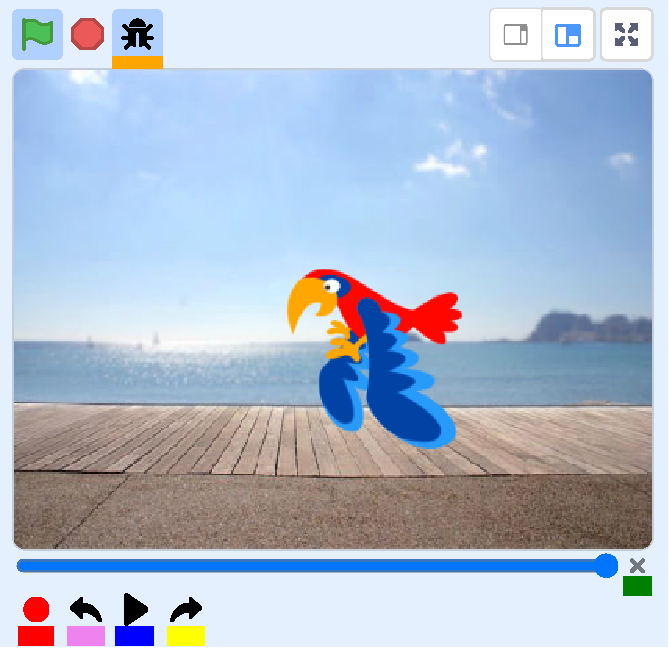
\includegraphics[width=\textwidth]{ide}
    \caption{
        Blink additions to the controls and canvas of the Scratch environment.
        The bug-shaped button (underlined in orange) enables and disables the debugger.
        It is the only Blink addition that is visible in the environment in normal mode.
        Other additions become visible when in debug mode.
        The back-in-time slider underneath the canvas shows the progress of the recording and allows users to jump back and replay the recording.
        The small button to the right of the slider (underlined in green) allows the user to clear the recording.
        The red dot (underlined in red) indicates if recording is active by blinking.
        The back, play/pause, and forward buttons (underlined in pink, blue and yellow) allow the user to control either the recording or the execution.
    }
    \label{fig:blink-ide}
\end{figure}

The Blink debugger is built on top of and adds extra functionality to the Scratch environment (\cref{fig:blink-ide}).
When the debugger is disabled, all functionalities of the base Scratch environment remain unchanged.
To activate (and deactivate) debug mode, the user must press the bug-shaped button above the canvas.
While the debugger is active, the navigation bar turns green as a visual aid.
This way, a clear distinction is made between the default Scratch execution mode and debug mode.

\subsection{Stepwise execution}\label{subsec:stepwise-execution}
While the debugger is active, the execution of the Scratch project can be paused.
In this state, execution can be continued in a stepwise manner, with the step button.
Pressing this button will execute exactly one block in all scripts for which there is a corresponding thread in the \texttt{Runtime} (see \cref{subsec:instrumentation-for-stepping}).
After each step, the execution will pause again.
This way, the programmer can execute the program at their own pace, providing greater understanding of the impact of each block on the program state and making it easier to identify where errors may occur.
To return to the normal execution of the program, the resume button can be used (the same button as the pause button: which changes shape based on the execution state).

To be able to closely follow how a Scratch program is executed, Blink highlights blocks in the workspace with a dark grey hue.
During the execution of the program, these are the next blocks that will be executed in each active script.
These blocks are also highlighted when replaying a recording of the program.

\subsection{Back-in-time debugging}\label{subsec:back-in-time-debugging}
Finally, Blink allows replaying the last execution (i.e.\ the recording) of a Scratch program, inspired by back-in-time debuggers.
These debuggers allow the programmer to go back in the execution, often by recording program execution~\autocite{barrTardisAffordableTimetravel2014,barrTimetravelDebuggingJavaScript2016,czaplickiAsynchronousFunctionalReactive2013,balzerEXDAMSExtendableDebugging1969,ungarDebuggingExperienceImmediacy1997,chenReversibleDebuggingUsing2001,crescenziReversibleExecutionVisualization2000}.
When the debugger is active, a recording is automatically made, as can be seen on the slider below the canvas.
Selecting a point on the slider or pressing the back button will pause execution, and the selected point in the recording will be restored.
This includes the entire visual state of all sprites and their clones.
While back-in-time debugging is a quite complex debugger feature, our experimental study in \cref{subsec:blink-experimental-study} shows that providing a simple video-player-like interface is intuitive for young students.

\subsection{Programmed breakpoints}\label{subsec:programmed-breakpoints}

\begin{varwidth}{0.2\linewidth}
    \begin{scratch}[scale=0.6]
        \blockdebug{pause}
    \end{scratch}
\end{varwidth}%
\hspace{1em}%
\begin{varwidth}{0.4\linewidth}
    \begin{scratch}[scale=0.6]
        \blockdebug{pause if \emptybooldebug}
    \end{scratch}
\end{varwidth}%
\hspace{1em}%
\begin{varwidth}{0.5\linewidth}
    \begin{scratch}[scale=0.6]
        \blockdebug{wait until \emptybooldebug{} and pause}
    \end{scratch}
\end{varwidth}%

Blink adds three custom blocks to Scratch to manually program breakpoints.
Additionally, \setscratch{scale=0.5}\booldebug{debugger is enabled?} reports whether the debugger is currently active or not.
When in debug mode, the execution of the pause block suspends the Scratch program.
In contrast, the pause block represents a conditional breakpoint that only pauses the execution if its corresponding condition evaluates to true.
The wait until and pause block waits until a condition holds and then suspends the execution.

\section{Software architecture}\label{sec:blink-software-architecture}

Internally, Scratch consists of several interconnected components implemented in JavaScript (\cref{sec:scratch-internal}).
However, for the integration of Blink, changes were only made in the virtual machine and the user interface.
The Blink debugger consists of three main components: instrumentation of the virtual machine for stepping, recording of the execution state, and the custom debug extension, which implements the breakpoints.

%\begin{figure}
%    \centering
%    \includestandalone[width=0.7\linewidth]{architecture}
%    \caption{
%        Diagram showing the internal interaction between the Scratch VM and Scratch GUI\@.
%    }
%    \label{fig:blink-architecture}
%\end{figure}

\subsection{Instrumentation for stepping}\label{subsec:instrumentation-for-stepping}

The virtual machine executes Scratch programs and preserves their current state.
It consists of three main modules relevant to the debugger: the \texttt{Runtime}, the \texttt{Sequencer}, and the \texttt{Execute} module.
The \texttt{Runtime} module maintains a list of active threads.
These objects embody the execution state of a script.
Threads are created when certain events trigger (i.e.\ a green flag is clicked), but can also be removed from the runtime (i.e.\ when deleting a clone).
A Scratch program is executed by repeatedly calling the \texttt{\_step} method of the \texttt{Runtime}, typically 30 times per second.
This method subsequently creates threads, destroys threads, and calls the \texttt{stepThreads} method of the \texttt{Sequencer}.
\texttt{stepThreads} will iterate all threads and ensure they are ready to be executed.
Finally, it will call the \texttt{execute} method of the \texttt{Execute} module for each thread, which will do the actual execution.

Blink implements the pause, step, and resume commands of the debugger by instrumenting the \texttt{\_step} method of the \texttt{Runtime}.
The instrumentation consists of injecting the code for recording state into this \texttt{\_step} method in the Blink fork of the Scratch virtual machine.
If the execution of the program is paused, no steps will be taken.
It is important to note that all other tasks performed by the \texttt{\_step} method will still be carried out.
Therefore, user actions will continue to result in the creation of threads, which will, however, not be executed.

If, on the other hand, the execution is paused, but a step is taken, the \texttt{\_step} method will execute one block for each active thread.
If the execution is not paused, the \texttt{\_step} method behaves as normal.

The definition of a step in Blink differs from the \texttt{\_step} method in the virtual machine and does not execute a single block, as the step functionality does in a traditional debugger.
This is a consequence of the Scratch execution model, which presents a dichotomy between code execution and user observable state.
The former is inherently sequential: the virtual machine executes one block after the other, decides when a thread switch is needed, and in what order threads are executed.
The latter is inherently concurrent: multiple sprites/clones act at the same time.

In Blink, we prioritize maintaining the observed concurrency by ensuring that when stepping through the code, all scripts advance simultaneously for focused debugging.
This approach allows users to keep focus on relevant scripts without distractions from visible thread switches or manual stepping, which can be cumbersome in complex programs.
Users can thus focus on the script(s) they believe are involved in the failure while ignoring (correct) scripts running at the same time.
We discuss this more in great depth in \cref{ch:scratch-execution-model}.

\subsection{Back-in-time debugging}\label{subsec:arch-back-in-time-debugging}
Blink also offers back-in-time debugging capabilities.
During a debugging session, it instruments the virtual machine and constructs a snapshot of the program state each time a step is executed.
These snapshots contain the entire state of the Scratch program, including the position of the sprites, the active blocks, clones, and the pen.
To implement this feature, we modified the \texttt{Execute} component (\cref{fig:blink-architecture}) to create a snapshot at the end of the \texttt{execute} method.
Once a debugging session has been completed, these snapshots can be consulted to restore the program state.

\subsection{Programmed breakpoints}\label{subsec:arch-programmed-breakpoints}
Pausing the execution of a running program by manually stepping and pausing the execution can rapidly become tiresome.
Therefore, many debuggers include the ability to set user-defined breakpoints.
In Blink, we have extended the block language to include four additional blocks to pause the execution of a program, to inspect whether the debugger is active and to stop the program based on a condition.

In our original design, we experimented with a large set of highly specific debugging blocks, for example, a block to stop execution when a sprite hits the wall.
However, we came to the conclusion that it would be impossible to account for every possible use-case.
Therefore, we decided it would be better to provide a small set of fundamental debugging blocks, which can be composed with existing Scratch blocks to express more specific debugging blocks.

\section{Examples}\label{sec:blink-illustrative-examples}

In this section, we give two illustrative examples to demonstrate how Blink assists in detecting bugs in Scratch programs.
The first project consists of guiding a sprite through a maze without going through the walls.
The second project is a typical logo exercise where a sprite needs to walk over a star figure without falling into the surrounding water.
These projects are typical Scratch exercises where we believe the debugger can be helpful in finding bugs easier and faster.

\subsection{\emph{Maze} exercise}\label{subsec:maze-exercise}

\begin{figure}
    \begin{wide}
        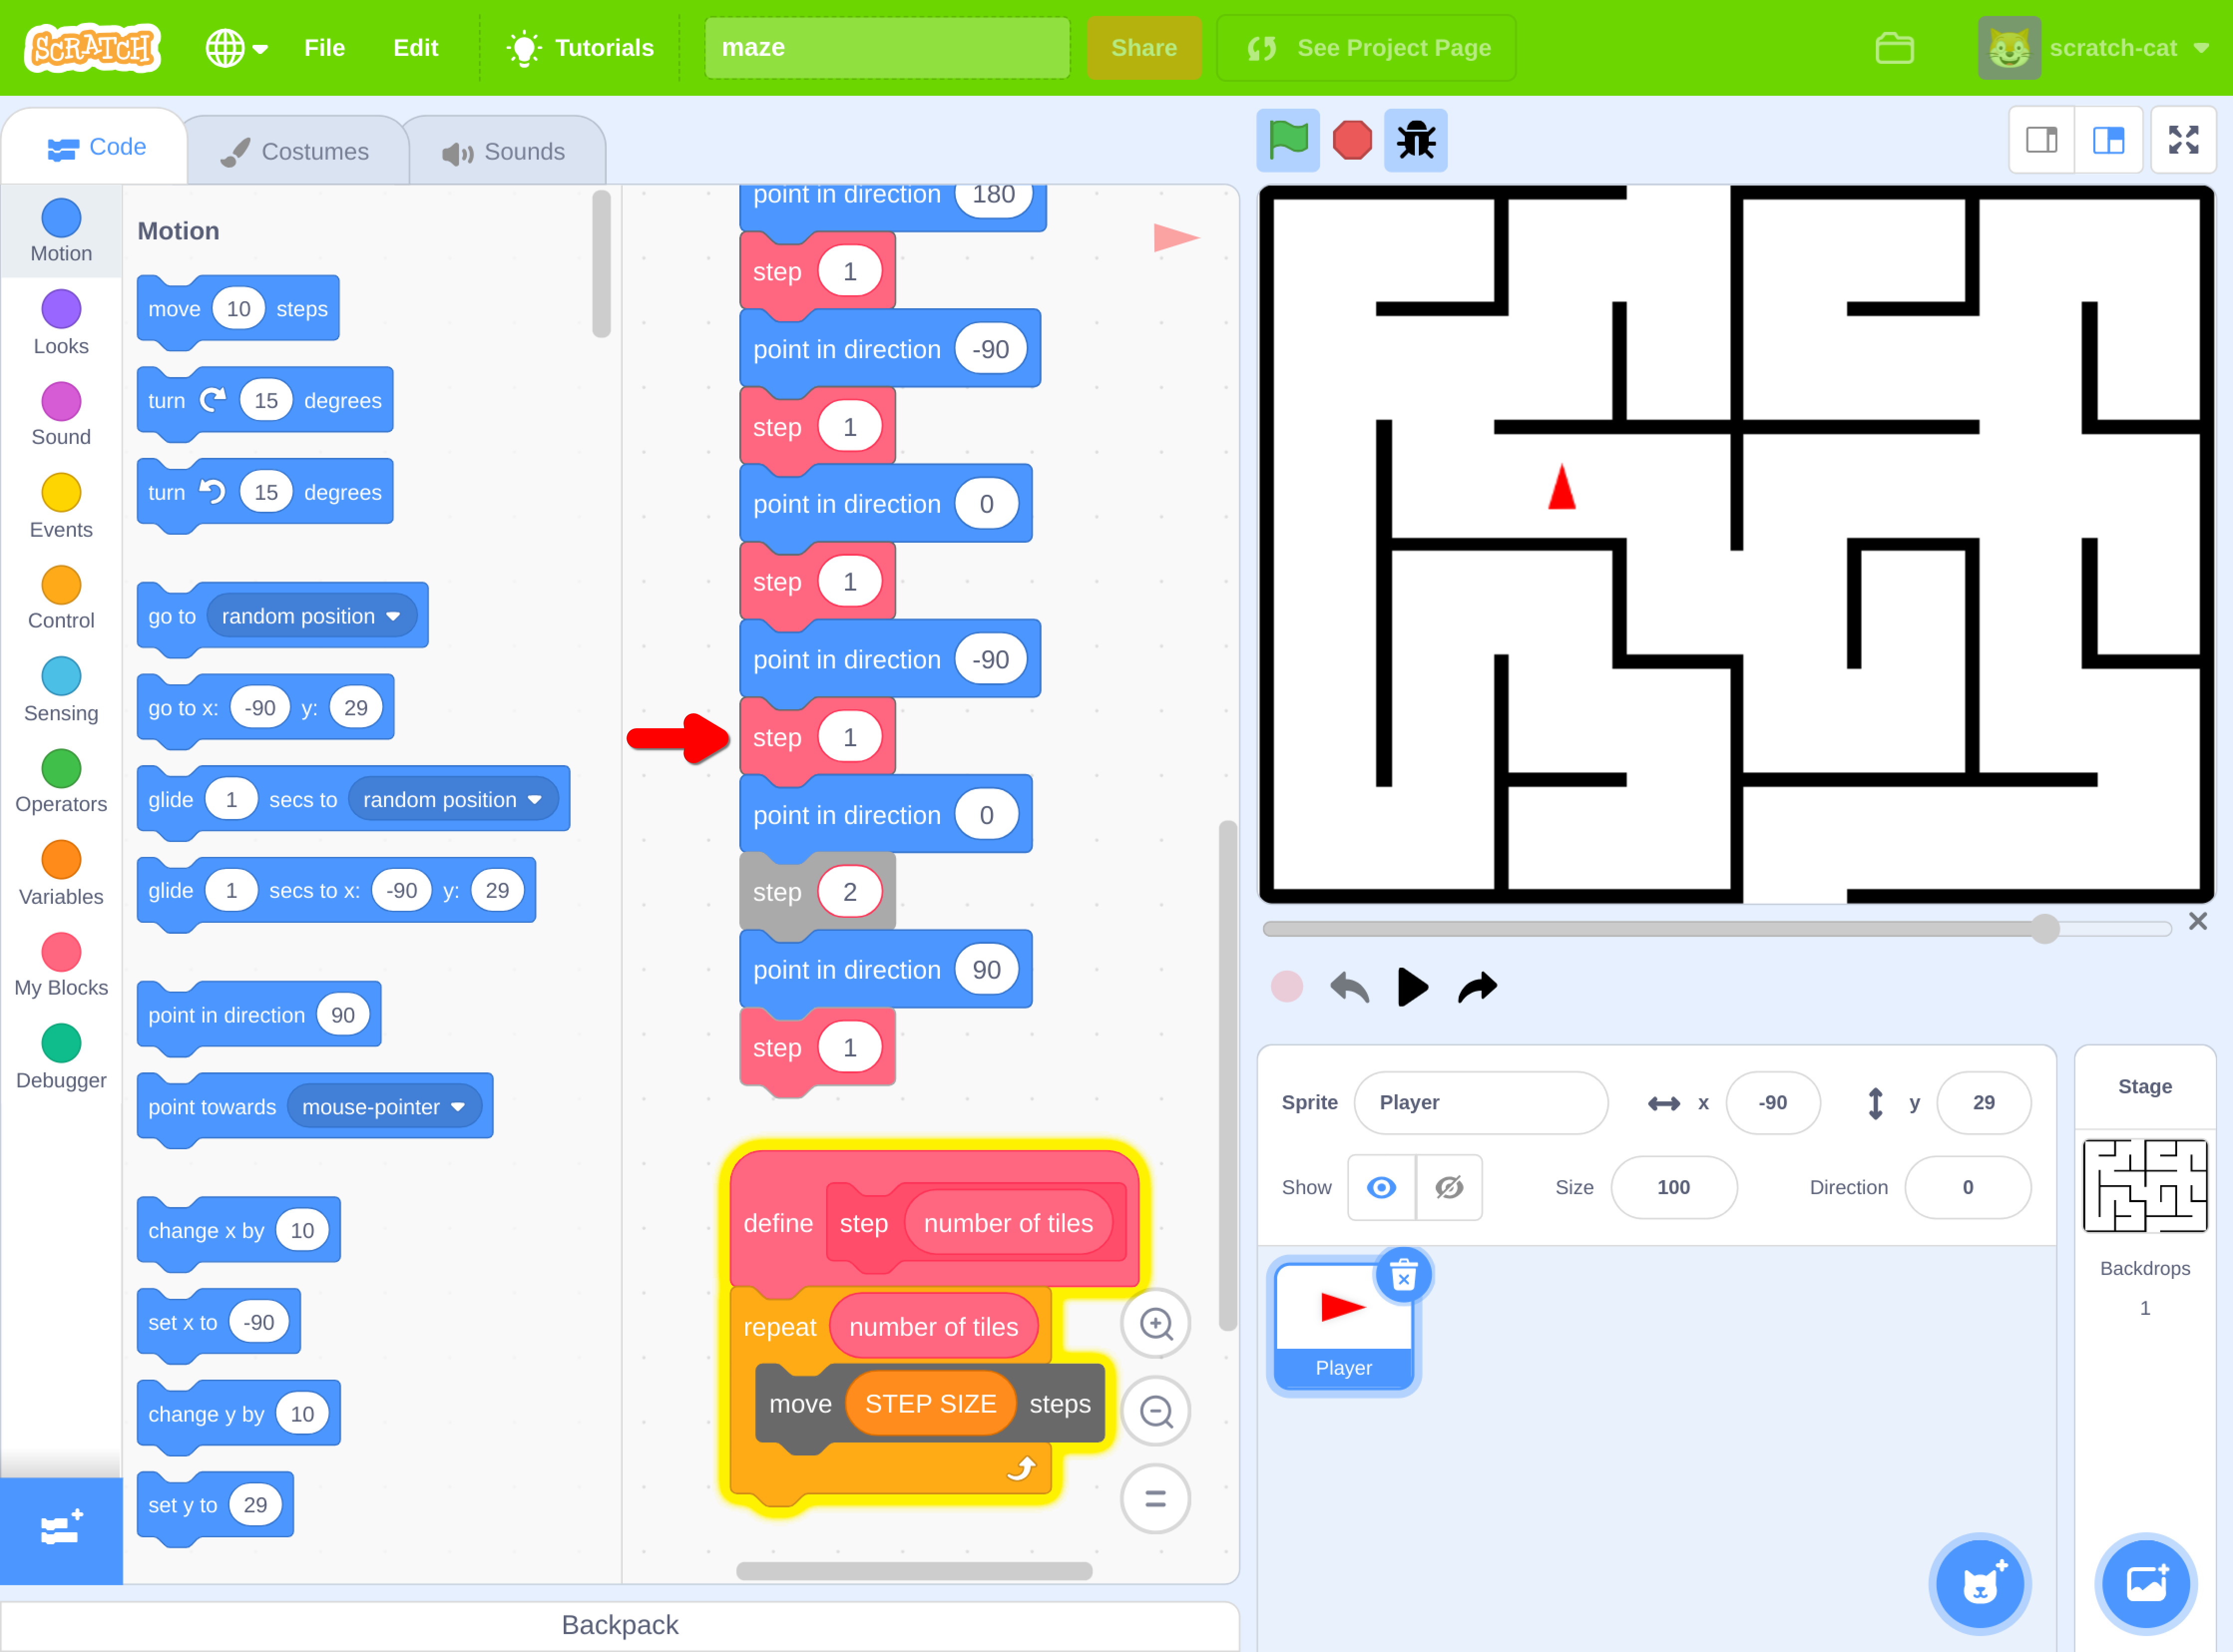
\includegraphics[width=\linewidth]{maze}
    \end{wide}
    \caption[The Maze exercise.]{
        The \emph{Maze} exercise.
        The execution is paused before the failure occurs.
        As indicated by the light grey colour, we are in the \scratchinline{\blockmoreblocks{step \ovalnum{2}}} block.
        The next block is the \scratchinline{\blockmove{move \ovalvariable{STEP SIZE} steps}} block, as indicated in dark grey.
        However, since the sprite Player is pointing upwards, it will go through the wall.
        The bug is in the \scratchinline{\blockmoreblocks{step \ovalnum{1}}} block indicated by the red arrow.
        The solution is to replace this block with a \scratchinline{\blockmoreblocks{step \ovalnum{2}}} block: in which case the Player would have moved one square more to the left, meaning the Player can go up without going through a wall.
        Note that further changes are needed to reach the exit of the maze.
    }
    \label{fig:maze}
\end{figure}

The \emph{Maze} exercise involves a single sprite in the shape of a red triangle representing the player.\footnote{\url{https://scratch.ugent.be/blink/editor?project=/blink/maze.sb3}}
The goal of the exercise is to write a program that navigates the player through the maze when the user presses the green flag.
Correctly navigating consists of not letting the player navigate through the walls of the maze.
In \cref{fig:maze} we show code, which seems to navigate the player through the maze correctly when executing the project.
Unfortunately, there is a small mistake towards the end of the solution, which is difficult to see when executing the program at full speed.
By making use of the debugger, it becomes easy to navigate through the execution of the program step-by-step, which makes it apparent where the player has taken a misstep.
Additionally, due to back-in-time debugging, it is easy to trace back to precisely where the bug emerged in the code.
With more traditional debuggers, which only provide step-wise execution, programmers frequently discover program errors too late, necessitating restarting the complete debugging session.

\subsection{\emph{Star} exercise}\label{subsec:star-exercise}

\begin{figure}
    \begin{wide}
        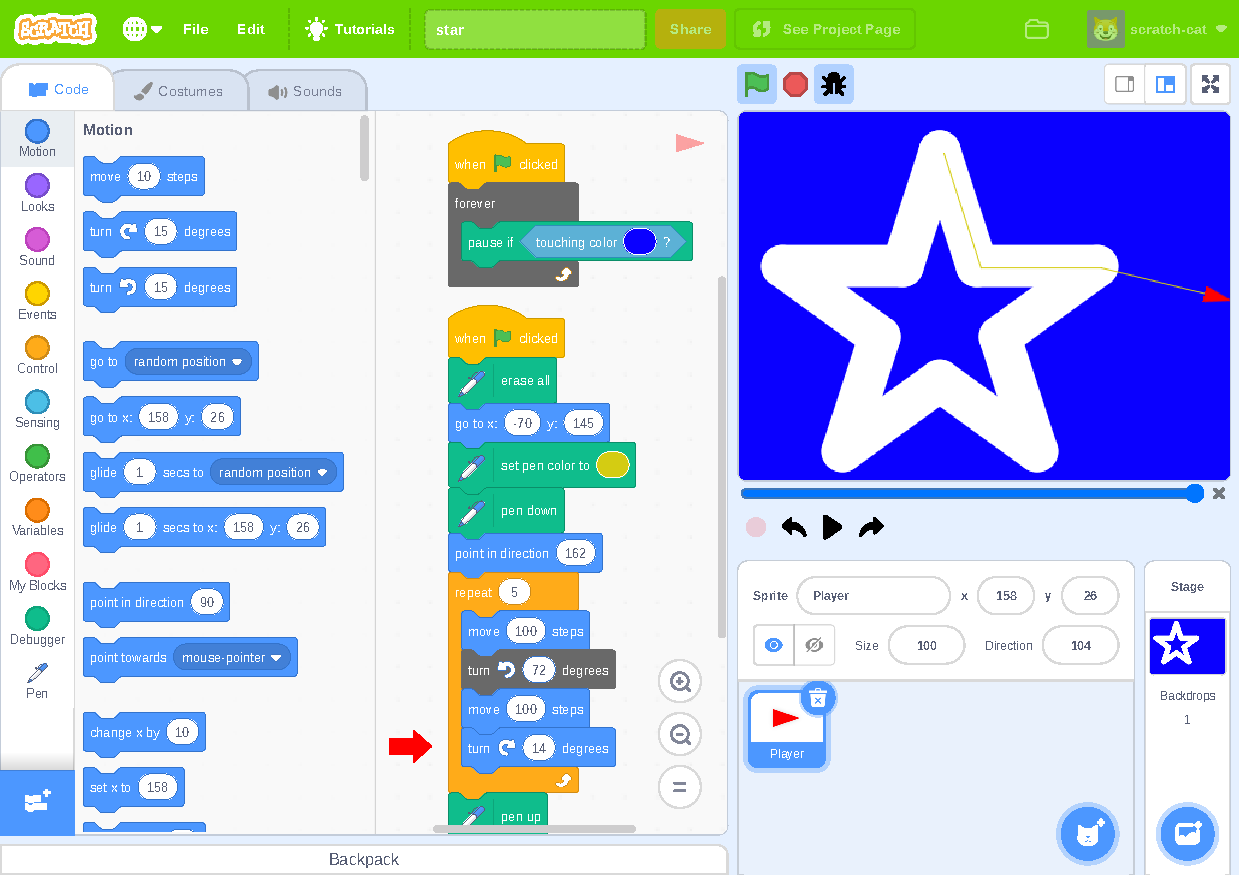
\includegraphics[width=\linewidth]{star}
    \end{wide}
    \caption[The Star exercise.]{
        The \emph{Star} exercise, which has two scripts.
        The bottom script contains a bug: the \scratchinline{\blockmove{turn \turnright{} \ovalnum{14} degrees}} block (red arrow) should be a \scratchinline{\blockmove{turn \turnright{} \ovalnum{144} degrees}} block.
        The top script helps to find the bug: once running, the code loops forever, evaluating the breakpoint each time, and pausing execution if the condition is true.
    }
    \label{fig:star-exercise}
\end{figure}

While the \emph{Maze} exercise demonstrates the capabilities of Blink in regard to step-wise execution and back-in-time debugging, the \emph{Star} exercise demonstrates the helpfulness of our custom debugging blocks.\footnote{\url{https://scratch.ugent.be/blink/editor?project=/blink/star.sb3}}
The aim of this exercise is to walk over a star-shaped figure surrounded by water.
Any program that directs the player into the water is buggy.
By making use of Blink's custom debugging blocks, it is quite easy to pause the execution of the program when the player touches something blue (\cref{fig:star-exercise}).
As soon as the green flag is clicked, the code repeatedly checks whether the player is touching something blue.
If it does, program execution is paused by using the \scratchinline{\blockdebug{pause if \emptybooldebug}} block.

\section{Impact}\label{sec:blink-impact}

\subsection{Related work}\label{subsec:related-work}
While most textual programming languages have debuggers, the emphasis in this chapter is on block-based languages.
In this domain (excluding Scratch), the most notable debuggers are the Microsoft MakeCode Arcade~\autocite{ballMicrosoftMakeCodeEmbedded2019} debugger and the Blockly debugger~\autocite{savidisCompleteBlockLevelVisual2020}.
Both of these debuggers offer basic debugging facilities, such as breakpoints, step functionality, and variable watches.
Unfortunately, these debuggers are not applicable to the Scratch environment because both MakeCode Arcade and Blockly assume a sequential execution model, while the Scratch programming language is inherently concurrent.
The Snap\textit{!} block-based programming language~\autocite{monigSnapBuildYour2024} does support concurrency, but its debugger lacks back-in-time debugging functionality.
Next to block-based programming languages, we have taken inspiration from back-in-time debuggers~\autocite{barrTardisAffordableTimetravel2014,barrTimetravelDebuggingJavaScript2016}.

For Scratch, we are aware of three existing debuggers.
The first provides pause/resume/step functionality and breakpoints~\autocite{wangDevelopingResourcesDebugging2021}.
The second debugger is a browser extension that provides breakpoints and advanced logging~\autocite{ScratchAddons2023}.
The last, and most recent, debugger is NuzzleBug~\autocite{deinerNuzzleBugDebuggingBlockBased2024}.
It provides similar functionality to Blink, but makes some different choices in its implementation and user interface.
For example, the step functionality in NuzzleBug is a more traditional step, advancing one block at a time.

The need for tools to help find bugs in Scratch projects is also illustrated by the existence of other tools.
These include multiple linter-style tools like Hairball~\autocite{boeHairballLintinspiredStatic2013}, Dr.\ Scratch~\autocite{moreno-leonDrScratchWeb2015}, QualityHound~\autocite{techapalokulQualityHoundOnline2017} and LitterBox~\autocite{fraserLitterBoxLinterScratch2021}, or test frameworks such as Whisker~\autocite{stahlbauerTestingScratchPrograms2019} and \textsc{itch}~\autocite{johnsonITCHIndividualTesting2016}.

\subsection{Experimental study}\label{subsec:blink-experimental-study}
To validate the usefulness of the debugger in helping students understand their code better, we conducted a quasi-experimental study~\autocite{shadishExperimentalQuasiexperimentalDesigns2002}.
The test group consisted of 16 students aged 8 to 11, which is at the lower end of Scratch's target audience.

Our experiment started with a short introduction explaining the different features of Blink and how they can be used.
Subsequently, we provided the students with two projects as discussed in \cref{sec:blink-illustrative-examples}.
Both projects contained an error leading to unwanted behaviour during the execution of the program.
During each exercise, we encouraged the students to make use of the features of the debugger to correct the implementation.

Our study aimed to determine the ease of use and usefulness of Blink.
Participants were asked to rate both aspects for three different aspects of the debugger tool: traditional debugger operations, usage of breakpoints, and back-in-time debugger.
A five-point scale, represented as a row of smiley faces, was provided for each statement.
The results of this questionnaire are shown in \cref{fig:blink-results}.

\begin{figure}
    % https://observablehq.com/d/b50757d4920f2318
    \centering
    \includestandalone{likert}
    \caption{
        Answers regarding the ease of use and the usefulness of the debugger in general,
        the breakpoints and the ability to go back in time to detect errors.
    }
    \label{fig:blink-results}
\end{figure}

The findings indicate unanimous agreement among participants that revisiting previous states is a straightforward and advantageous approach for identifying errors in Scratch code.
The custom breakpoints were less intuitive for most students and received a lower score on ease of use.
While breakpoints were conceptually clear to most students, when they were asked to implement a custom breakpoint to pause the execution, many of them struggled.
Finally, if we look at the score distributions for the debugger in general, we can see that they embody the combination of the distributions for the usage of the breakpoints and the ability to go back in time.

\section{Conclusions}\label{sec:blink-conclusions}
In this chapter we introduced Blink, a debugger for the Scratch programming language.
Blink offers stepwise execution, back-in-time debugging, and the ability to define custom breakpoints.
These features allow students to closely follow the execution of their programs and consequently make it easier to find errors.
To evaluate the effectiveness of our debugger, we conducted a quasi-experimental study.
The results of this study show that most aspects of the debugger are both useful and easy to use.
We observed a strong preference for back-in-time debugging and observed that custom breakpoints are less intuitive than back-in-time debugging.
In future work, we will focus on inventing novel user interface elements to further improve the ease of use for programming custom breakpoints for students.

\end{document}
